\question{نمونه‌ی جدول و شکل}

این فایل برای نمایش جدول‌ها و شکل‌هاست.
اگر نام فایل شکل را عوض کردید، کافی است مسیر را در
\begin{latin}
	\texttt{\textbackslash includegraphics}
\end{latin}
تغییر دهید.

\subsection{جدول}
نمونه‌ی یک جدول با ستون‌های ترکیبی (نیازمند \lr{array} که در قالب فعال است).
برای جدول‌های انگلیسی، می‌توانید از یک بلوک \lr{LTR} هم استفاده کنید:

\begin{table}[H]
	\centering
	\renewcommand{\arraystretch}{1.4}
	\begin{tabular}{|c|>{\raggedright\arraybackslash}p{10.5cm}|}
		\hline
		\lr{Item}    & توضیح                                         \\
		\hline
		\(O(n)\)     & مرتبه‌ی خطی؛ مثلاً پیمایش یک آرایه              \\
		\hline
		\(\poly(n)\) & یک چندجمله‌ای از \(n\) (برای تحلیل الگوریتم‌ها) \\
		\hline
	\end{tabular}
\end{table}

\begin{LTR}
	\begin{table}[H]
		\centering
		\begin{tabular}{|l|l|}
			\hline
			\lr{Key}  & \lr{Meaning}      \\
			\hline
			\lr{n}    & \lr{input size}   \\
			\lr{T(n)} & \lr{running time} \\
			\hline
		\end{tabular}
		\caption{An LTR table example}
	\end{table}
\end{LTR}

\subsection{شکل}
نمونه‌ی یک شکل (از فایل‌های موجود در \lr{assets/}).
این الگو عمداً یک فایل موجود را استفاده می‌کند تا روی سیستم‌های مختلف بدون دردسر کامپایل شود.

\begin{figure}[H]
	\centering
	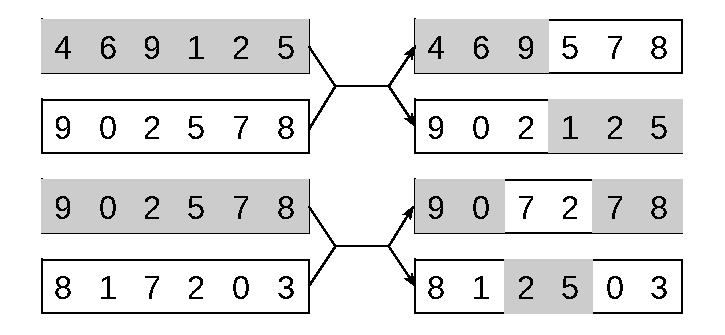
\includegraphics[width=0.55\textwidth]{assets/crossover_diagram.pdf}
	\caption{یک نمونه شکل برای قرار دادن تصویر/دیاگرام}
\end{figure}

اگر شکل انگلیسی بود و خواستید کپشن انگلیسی بنویسید:
\begin{latin}
	\textit{You can also write English captions in a latin block.}
\end{latin}

\subsection{لیست‌ها (نمونه)}
گاهی می‌خواهید مراحل را با حروف فارسی شماره‌گذاری کنید:
\begin{الفبا}
\item آماده‌سازی داده‌ها
\item رسم شکل/جدول
\item نتیجه‌گیری
\end{الفبا}

